\clearpage
\SourceLeaf{100}%

\begin{center}
\large UNTERSUCHUNGEN\\
ÜBER DIE TRANSCENDENTEN FUNCTIONEN, DIE AUS DEM\\
INTEGRAL $\displaystyle\int \frac{dx}{\BareRoot{(1+x^3)}}$ IHREN URSPRUNG HABEN.
\end{center}



\noindent\hspace*{\parindent}Man bezeichne den Werth des Integrals $\int \frac{dx}{\BareRoot{(1+x^3)}}$ von $x=-1$ bis zu
$x=z$ allgemein durch $\Pi z$; umgekehrt, wenn $\Pi z=y$, setze man $z=\boldsymbol{P}y$.
Dann ist $\boldsymbol{P}$ eine einförmige und zwar periodische Function von $y$, welche
durch folgendes Schema sinnlich gemacht werden kann:

\begin{center}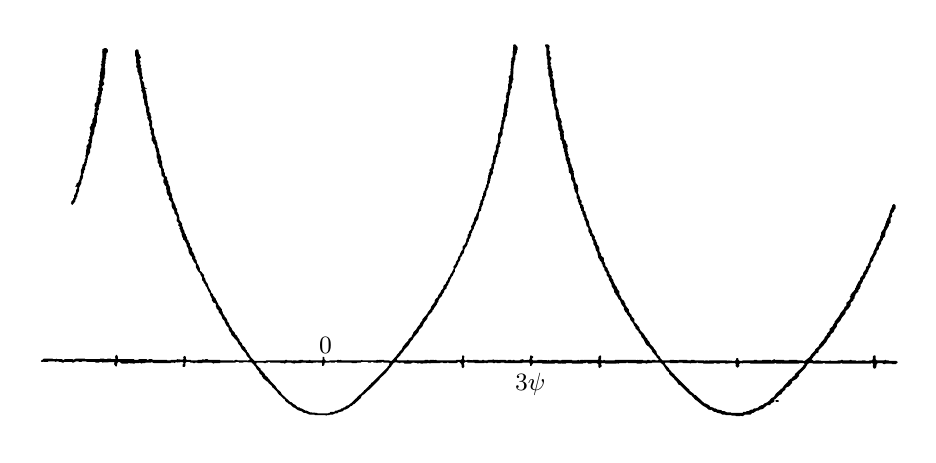
\begin{tikzpicture}[x=.2pt,y=-.2pt]
\path[use as bounding box] (0,0) rectangle (1590,735);
\path[fill=black,even odd rule]
(1351,674) -- (1352,676) -- (1357,676) -- (1357,674) -- (1356,673) -- (1352,673) -- cycle
(142,37) -- (139,37) -- (135,39) -- (135,43) -- (134,44) -- (135,45) -- (135,55) -- (134,56) -- (134,60) -- (133,61) -- (134,65) -- (132,67) -- (133,68) -- (133,73) -- (132,74) -- (132,79) -- (131,80) -- (131,85) -- (130,86) -- (130,88) -- (131,89) -- (131,93) -- (129,97) -- (130,98) -- (129,99) -- (130,101) -- (128,103) -- (129,105) -- (129,108) -- (127,109) -- (127,113) -- (128,114) -- (128,116) -- (127,117) -- (127,123) -- (125,125) -- (124,134) -- (121,138) -- (121,142) -- (123,144) -- (121,147) -- (121,153) -- (120,155) -- (122,156) -- (120,158) -- (120,161) -- (117,166) -- (117,172) -- (114,175) -- (114,178) -- (112,180) -- (114,188) -- (112,190) -- (113,192) -- (112,196) -- (111,197) -- (111,199) -- (112,200) -- (109,203) -- (110,205) -- (110,209) -- (106,214) -- (107,218) -- (106,219) -- (105,230) -- (104,231) -- (105,235) -- (103,238) -- (103,242) -- (102,243) -- (102,245) -- (99,248) -- (99,251) -- (96,258) -- (96,266) -- (94,270) -- (95,271) -- (94,272) -- (94,274) -- (92,277) -- (92,279) -- (88,282) -- (88,284) -- (86,287) -- (86,288) -- (88,287) -- (90,289) -- (90,290) -- (88,292) -- (87,298) -- (84,303) -- (84,307) -- (82,309) -- (82,311) -- (79,314) -- (79,316) -- (78,317) -- (80,320) -- (81,320) -- (86,314) -- (86,311) -- (88,309) -- (88,307) -- (90,305) -- (90,301) -- (93,294) -- (93,289) -- (97,281) -- (97,277) -- (100,271) -- (99,270) -- (100,269) -- (100,266) -- (99,265) -- (101,263) -- (102,261) -- (102,258) -- (104,256) -- (104,251) -- (106,248) -- (106,245) -- (107,244) -- (107,240) -- (108,239) -- (109,232) -- (113,225) -- (113,219) -- (115,216) -- (115,209) -- (116,208) -- (117,197) -- (120,191) -- (121,181) -- (123,178) -- (123,175) -- (125,171) -- (125,159) -- (127,157) -- (126,151) -- (129,147) -- (128,144) -- (129,143) -- (129,140) -- (132,135) -- (132,131) -- (133,130) -- (132,128) -- (132,125) -- (133,124) -- (133,121) -- (134,120) -- (134,115) -- (136,113) -- (136,110) -- (134,107) -- (138,103) -- (138,100) -- (136,96) -- (137,95) -- (137,93) -- (139,91) -- (139,85) -- (140,84) -- (140,73) -- (139,72) -- (140,68) -- (139,66) -- (141,64) -- (140,61) -- (141,60) -- (141,57) -- (142,56) -- (141,54) -- (142,52) -- (142,47) -- (145,44) -- (145,40) -- cycle
(1568,321) -- (1566,319) -- (1564,319) -- (1562,321) -- (1562,323) -- (1558,331) -- (1558,334) -- (1557,335) -- (1555,343) -- (1553,345) -- (1553,347) -- (1551,350) -- (1551,352) -- (1550,353) -- (1549,358) -- (1547,361) -- (1547,363) -- (1542,370) -- (1542,374) -- (1540,378) -- (1540,381) -- (1538,385) -- (1534,390) -- (1533,395) -- (1528,405) -- (1528,407) -- (1522,417) -- (1520,425) -- (1518,427) -- (1518,430) -- (1515,432) -- (1514,437) -- (1510,442) -- (1509,447) -- (1505,451) -- (1504,453) -- (1504,456) -- (1501,459) -- (1497,467) -- (1497,469) -- (1495,471) -- (1495,473) -- (1487,482) -- (1487,484) -- (1485,486) -- (1487,488) -- (1484,493) -- (1479,497) -- (1479,502) -- (1477,504) -- (1476,504) -- (1475,508) -- (1469,515) -- (1466,521) -- (1458,531) -- (1458,533) -- (1455,537) -- (1455,539) -- (1449,544) -- (1449,547) -- (1448,549) -- (1444,553) -- (1444,555) -- (1440,559) -- (1440,561) -- (1438,563) -- (1438,564) -- (1433,569) -- (1433,570) -- (1430,573) -- (1429,576) -- (1423,581) -- (1422,584) -- (1416,590) -- (1413,595) -- (1404,602) -- (1401,602) -- (1400,601) -- (1391,601) -- (1390,600) -- (1376,600) -- (1375,601) -- (1367,601) -- (1366,600) -- (1350,600) -- (1349,599) -- (1345,601) -- (1343,601) -- (1342,600) -- (1328,600) -- (1327,601) -- (1318,601) -- (1317,600) -- (1313,600) -- (1312,601) -- (1292,601) -- (1291,602) -- (1286,602) -- (1284,600) -- (1284,598) -- (1283,597) -- (1281,597) -- (1280,598) -- (1280,600) -- (1278,602) -- (1272,602) -- (1271,601) -- (1269,602) -- (1267,601) -- (1265,602) -- (1263,601) -- (1231,601) -- (1230,602) -- (1228,601) -- (1225,601) -- (1223,602) -- (1222,601) -- (1205,601) -- (1204,600) -- (1199,600) -- (1198,601) -- (1192,601) -- (1191,600) -- (1177,600) -- (1176,601) -- (1161,600) -- (1160,601) -- (1147,601) -- (1143,597) -- (1142,594) -- (1141,594) -- (1137,590) -- (1136,585) -- (1131,579) -- (1131,578) -- (1125,572) -- (1123,567) -- (1120,564) -- (1119,561) -- (1117,560) -- (1113,553) -- (1107,547) -- (1105,543) -- (1105,541) -- (1101,537) -- (1101,536) -- (1096,532) -- (1096,526) -- (1091,521) -- (1091,519) -- (1088,516) -- (1086,512) -- (1086,509) -- (1081,503) -- (1080,501) -- (1080,498) -- (1078,496) -- (1078,494) -- (1076,492) -- (1075,492) -- (1072,488) -- (1072,486) -- (1069,482) -- (1069,476) -- (1066,473) -- (1064,468) -- (1062,466) -- (1058,458) -- (1058,456) -- (1055,452) -- (1055,449) -- (1051,445) -- (1051,442) -- (1048,437) -- (1048,435) -- (1044,431) -- (1043,425) -- (1041,423) -- (1041,416) -- (1036,412) -- (1036,409) -- (1033,404) -- (1033,398) -- (1031,394) -- (1029,392) -- (1029,389) -- (1027,386) -- (1027,384) -- (1024,381) -- (1025,380) -- (1025,378) -- (1020,371) -- (1020,368) -- (1015,358) -- (1014,350) -- (1010,343) -- (1010,340) -- (1008,336) -- (1008,333) -- (1005,330) -- (1005,325) -- (1004,324) -- (1004,321) -- (1000,318) -- (1001,316) -- (1001,313) -- (998,310) -- (998,307) -- (994,298) -- (994,296) -- (995,295) -- (994,293) -- (995,291) -- (994,289) -- (994,285) -- (990,280) -- (989,273) -- (987,269) -- (987,263) -- (986,262) -- (987,260) -- (985,257) -- (985,255) -- (983,251) -- (983,248) -- (980,244) -- (981,243) -- (980,242) -- (980,237) -- (977,233) -- (977,231) -- (978,230) -- (976,227) -- (976,224) -- (975,223) -- (975,220) -- (976,219) -- (975,218) -- (975,216) -- (976,214) -- (975,213) -- (975,211) -- (973,209) -- (973,206) -- (969,201) -- (969,193) -- (968,192) -- (969,188) -- (968,187) -- (968,185) -- (966,183) -- (966,178) -- (964,175) -- (965,169) -- (964,168) -- (963,164) -- (961,162) -- (961,158) -- (960,157) -- (959,148) -- (955,139) -- (957,131) -- (954,125) -- (953,110) -- (951,108) -- (951,95) -- (948,90) -- (948,88) -- (949,87) -- (948,82) -- (949,80) -- (947,77) -- (947,74) -- (946,73) -- (946,70) -- (945,69) -- (945,66) -- (946,64) -- (944,62) -- (945,58) -- (946,57) -- (946,54) -- (943,51) -- (943,48) -- (944,47) -- (944,43) -- (942,41) -- (943,33) -- (940,30) -- (936,30) -- (935,31) -- (935,33) -- (937,37) -- (937,50) -- (938,51) -- (938,56) -- (939,57) -- (939,67) -- (940,68) -- (939,74) -- (941,76) -- (941,86) -- (943,90) -- (944,100) -- (945,101) -- (944,103) -- (944,106) -- (945,107) -- (945,112) -- (947,115) -- (947,122) -- (949,126) -- (949,131) -- (950,132) -- (950,137) -- (951,138) -- (952,147) -- (954,150) -- (954,160) -- (955,161) -- (955,165) -- (958,170) -- (958,178) -- (959,179) -- (959,184) -- (962,189) -- (961,191) -- (962,193) -- (962,196) -- (963,197) -- (962,201) -- (966,206) -- (965,208) -- (967,211) -- (967,216) -- (969,220) -- (969,224) -- (970,225) -- (970,228) -- (971,229) -- (971,232) -- (972,233) -- (972,238) -- (974,242) -- (974,245) -- (977,248) -- (976,249) -- (976,251) -- (977,252) -- (978,262) -- (980,263) -- (982,267) -- (982,274) -- (986,281) -- (986,285) -- (987,286) -- (987,291) -- (988,292) -- (988,295) -- (992,301) -- (992,308) -- (994,310) -- (994,314) -- (995,315) -- (996,319) -- (998,321) -- (998,325) -- (1000,328) -- (1000,331) -- (1002,332) -- (1002,336) -- (1004,339) -- (1004,341) -- (1006,343) -- (1006,347) -- (1008,350) -- (1010,359) -- (1011,359) -- (1013,362) -- (1013,368) -- (1016,373) -- (1016,376) -- (1017,376) -- (1019,378) -- (1020,383) -- (1022,386) -- (1022,391) -- (1025,395) -- (1027,403) -- (1029,405) -- (1031,416) -- (1033,418) -- (1034,421) -- (1037,424) -- (1037,426) -- (1039,428) -- (1039,431) -- (1042,435) -- (1042,438) -- (1046,443) -- (1046,447) -- (1050,452) -- (1050,456) -- (1052,458) -- (1055,464) -- (1055,467) -- (1059,473) -- (1060,479) -- (1062,480) -- (1062,482) -- (1065,485) -- (1068,491) -- (1070,492) -- (1073,500) -- (1077,505) -- (1077,508) -- (1080,514) -- (1082,515) -- (1083,518) -- (1088,524) -- (1089,528) -- (1094,534) -- (1096,539) -- (1098,541) -- (1098,543) -- (1104,549) -- (1104,551) -- (1108,555) -- (1109,559) -- (1112,562) -- (1117,572) -- (1120,575) -- (1121,575) -- (1128,583) -- (1128,585) -- (1136,594) -- (1136,595) -- (1140,599) -- (1140,600) -- (1139,601) -- (1134,601) -- (1133,600) -- (1129,600) -- (1128,601) -- (1124,601) -- (1123,600) -- (1120,600) -- (1119,601) -- (1112,601) -- (1111,600) -- (1105,600) -- (1104,601) -- (1103,600) -- (1101,600) -- (1100,601) -- (1098,600) -- (1062,600) -- (1061,601) -- (1043,601) -- (1041,600) -- (1040,601) -- (1037,601) -- (1035,599) -- (1036,598) -- (1036,593) -- (1034,592) -- (1031,595) -- (1031,599) -- (1030,600) -- (1005,600) -- (1004,601) -- (1003,600) -- (999,600) -- (998,601) -- (996,601) -- (995,600) -- (993,601) -- (984,601) -- (983,600) -- (965,600) -- (964,601) -- (959,601) -- (958,600) -- (947,600) -- (946,601) -- (942,601) -- (941,600) -- (940,601) -- (922,600) -- (921,601) -- (913,601) -- (911,599) -- (911,598) -- (913,596) -- (913,594) -- (909,592) -- (908,593) -- (907,599) -- (905,601) -- (904,600) -- (898,601) -- (894,599) -- (890,600) -- (889,601) -- (880,601) -- (879,600) -- (877,600) -- (876,601) -- (874,601) -- (873,600) -- (869,600) -- (868,601) -- (864,601) -- (863,600) -- (853,600) -- (851,601) -- (850,600) -- (842,600) -- (841,599) -- (840,600) -- (832,600) -- (831,601) -- (825,601) -- (824,600) -- (822,600) -- (821,601) -- (815,601) -- (814,600) -- (805,600) -- (804,601) -- (794,600) -- (793,601) -- (790,601) -- (788,599) -- (789,594) -- (787,592) -- (786,592) -- (785,593) -- (785,598) -- (783,600) -- (775,600) -- (774,601) -- (739,601) -- (738,600) -- (736,600) -- (735,601) -- (733,600) -- (727,600) -- (726,601) -- (724,601) -- (723,600) -- (718,600) -- (717,601) -- (688,601) -- (687,600) -- (686,601) -- (668,601) -- (667,600) -- (667,598) -- (674,591) -- (674,590) -- (678,586) -- (681,581) -- (688,574) -- (692,567) -- (696,563) -- (697,560) -- (706,550) -- (707,546) -- (713,540) -- (716,533) -- (722,526) -- (722,524) -- (724,520) -- (731,513) -- (731,511) -- (734,508) -- (734,507) -- (740,499) -- (740,497) -- (742,495) -- (742,493) -- (744,489) -- (749,484) -- (749,482) -- (752,478) -- (753,474) -- (757,471) -- (757,468) -- (760,464) -- (760,462) -- (762,460) -- (763,456) -- (766,450) -- (768,448) -- (770,443) -- (772,441) -- (772,436) -- (775,432) -- (778,426) -- (778,424) -- (780,422) -- (782,418) -- (782,415) -- (785,412) -- (785,410) -- (788,407) -- (789,401) -- (791,397) -- (793,395) -- (795,391) -- (795,388) -- (797,386) -- (797,383) -- (800,379) -- (800,377) -- (801,376) -- (801,372) -- (803,370) -- (803,368) -- (806,363) -- (806,361) -- (810,353) -- (810,351) -- (814,346) -- (816,333) -- (818,331) -- (819,331) -- (820,324) -- (823,318) -- (823,314) -- (825,311) -- (825,308) -- (828,303) -- (829,295) -- (831,292) -- (831,290) -- (833,288) -- (833,283) -- (835,280) -- (835,277) -- (836,276) -- (836,273) -- (837,272) -- (837,268) -- (839,266) -- (841,262) -- (840,257) -- (842,255) -- (843,247) -- (845,245) -- (846,235) -- (848,233) -- (848,229) -- (850,227) -- (851,217) -- (853,215) -- (853,213) -- (852,212) -- (855,208) -- (854,206) -- (854,200) -- (858,193) -- (858,184) -- (860,182) -- (860,175) -- (861,174) -- (861,171) -- (863,167) -- (863,163) -- (866,158) -- (866,152) -- (867,151) -- (866,147) -- (868,144) -- (870,123) -- (871,122) -- (871,119) -- (872,118) -- (872,113) -- (875,108) -- (874,102) -- (876,99) -- (876,96) -- (878,93) -- (877,91) -- (878,68) -- (879,67) -- (879,63) -- (880,62) -- (880,59) -- (881,58) -- (881,50) -- (883,48) -- (883,46) -- (884,45) -- (884,41) -- (885,40) -- (885,35) -- (881,30) -- (879,30) -- (877,32) -- (878,33) -- (877,35) -- (877,42) -- (876,43) -- (876,46) -- (877,48) -- (876,49) -- (876,53) -- (874,55) -- (874,60) -- (873,61) -- (873,64) -- (874,65) -- (873,66) -- (873,74) -- (872,75) -- (873,77) -- (872,79) -- (872,85) -- (869,88) -- (869,90) -- (870,91) -- (870,95) -- (869,96) -- (869,98) -- (870,100) -- (868,102) -- (868,111) -- (867,112) -- (867,116) -- (865,118) -- (865,122) -- (864,123) -- (864,126) -- (865,127) -- (865,129) -- (864,130) -- (864,134) -- (861,139) -- (861,146) -- (860,147) -- (860,153) -- (859,154) -- (859,161) -- (857,163) -- (858,166) -- (856,168) -- (856,175) -- (855,176) -- (855,179) -- (854,180) -- (853,188) -- (850,192) -- (850,203) -- (849,204) -- (849,208) -- (846,214) -- (846,220) -- (843,226) -- (843,230) -- (841,232) -- (841,238) -- (840,239) -- (840,244) -- (838,247) -- (838,252) -- (834,257) -- (835,260) -- (833,263) -- (833,266) -- (832,267) -- (832,271) -- (831,272) -- (831,276) -- (830,277) -- (830,282) -- (828,285) -- (828,288) -- (826,291) -- (826,294) -- (824,296) -- (824,298) -- (823,299) -- (823,303) -- (821,305) -- (821,310) -- (819,311) -- (818,313) -- (818,316) -- (816,320) -- (817,321) -- (815,324) -- (815,327) -- (814,328) -- (813,333) -- (811,336) -- (810,340) -- (807,344) -- (806,350) -- (804,353) -- (804,355) -- (801,359) -- (802,363) -- (797,369) -- (797,372) -- (795,374) -- (795,379) -- (793,381) -- (792,387) -- (790,391) -- (786,395) -- (786,401) -- (784,403) -- (781,409) -- (781,411) -- (778,414) -- (777,419) -- (774,423) -- (773,427) -- (769,432) -- (770,435) -- (766,443) -- (764,445) -- (763,449) -- (760,452) -- (759,456) -- (756,460) -- (756,462) -- (751,467) -- (751,470) -- (750,472) -- (747,475) -- (746,478) -- (742,483) -- (741,487) -- (737,490) -- (735,494) -- (736,495) -- (729,504) -- (728,508) -- (723,514) -- (722,517) -- (713,527) -- (713,529) -- (709,534) -- (708,537) -- (705,540) -- (702,545) -- (697,550) -- (696,554) -- (694,556) -- (694,558) -- (688,563) -- (688,565) -- (681,572) -- (681,573) -- (678,576) -- (676,581) -- (671,586) -- (671,587) -- (667,591) -- (667,592) -- (658,602) -- (654,602) -- (653,601) -- (644,601) -- (643,600) -- (635,600) -- (634,601) -- (632,600) -- (630,601) -- (605,601) -- (604,600) -- (602,601) -- (567,601) -- (566,600) -- (563,601) -- (562,600) -- (560,600) -- (559,601) -- (546,601) -- (545,602) -- (539,602) -- (536,599) -- (536,596) -- (535,595) -- (533,595) -- (533,600) -- (532,601) -- (511,601) -- (510,600) -- (508,601) -- (498,601) -- (497,600) -- (492,600) -- (491,601) -- (488,601) -- (487,602) -- (485,601) -- (480,601) -- (478,602) -- (477,601) -- (469,601) -- (468,600) -- (466,600) -- (465,601) -- (431,601) -- (430,602) -- (410,602) -- (403,595) -- (399,588) -- (396,585) -- (396,583) -- (394,581) -- (393,578) -- (388,574) -- (387,570) -- (383,566) -- (383,564) -- (379,559) -- (379,557) -- (375,554) -- (374,551) -- (370,547) -- (368,542) -- (366,540) -- (364,536) -- (364,534) -- (361,531) -- (361,529) -- (359,525) -- (356,522) -- (355,519) -- (353,517) -- (352,513) -- (351,512) -- (351,509) -- (344,500) -- (344,498) -- (342,496) -- (342,494) -- (340,492) -- (340,490) -- (335,484) -- (335,482) -- (331,478) -- (331,476) -- (327,469) -- (325,462) -- (323,460) -- (321,456) -- (321,454) -- (318,450) -- (319,449) -- (319,447) -- (315,443) -- (315,442) -- (311,439) -- (311,435) -- (308,428) -- (306,426) -- (305,420) -- (303,418) -- (303,414) -- (301,412) -- (301,410) -- (299,406) -- (297,404) -- (297,399) -- (293,394) -- (293,390) -- (291,388) -- (291,385) -- (288,382) -- (288,379) -- (286,376) -- (286,374) -- (284,372) -- (283,367) -- (281,364) -- (281,362) -- (279,358) -- (279,354) -- (274,347) -- (274,342) -- (273,341) -- (273,338) -- (272,337) -- (272,335) -- (270,333) -- (270,327) -- (268,326) -- (267,321) -- (263,313) -- (263,310) -- (261,307) -- (261,302) -- (260,301) -- (260,299) -- (258,297) -- (257,288) -- (254,282) -- (254,278) -- (252,275) -- (252,271) -- (251,269) -- (250,269) -- (248,267) -- (248,263) -- (246,260) -- (246,256) -- (244,253) -- (244,250) -- (243,249) -- (243,242) -- (241,239) -- (241,233) -- (238,227) -- (238,223) -- (237,222) -- (237,219) -- (235,216) -- (234,207) -- (233,206) -- (233,204) -- (231,202) -- (231,198) -- (229,195) -- (229,192) -- (228,191) -- (228,183) -- (225,180) -- (225,178) -- (224,177) -- (225,175) -- (225,169) -- (223,166) -- (223,163) -- (224,162) -- (222,158) -- (222,155) -- (219,151) -- (220,149) -- (220,145) -- (217,140) -- (217,136) -- (216,135) -- (217,134) -- (216,132) -- (216,124) -- (215,123) -- (215,120) -- (214,119) -- (214,115) -- (212,112) -- (213,110) -- (216,110) -- (215,109) -- (213,109) -- (211,107) -- (210,99) -- (206,94) -- (208,92) -- (208,89) -- (207,88) -- (207,82) -- (206,81) -- (206,74) -- (204,72) -- (205,68) -- (203,66) -- (204,61) -- (202,58) -- (202,57) -- (205,54) -- (203,51) -- (203,49) -- (201,47) -- (200,40) -- (197,39) -- (194,42) -- (194,51) -- (196,53) -- (196,64) -- (197,65) -- (196,71) -- (198,73) -- (198,79) -- (200,82) -- (200,85) -- (202,87) -- (202,93) -- (203,94) -- (204,102) -- (205,103) -- (205,108) -- (206,109) -- (206,112) -- (205,113) -- (208,119) -- (208,126) -- (210,130) -- (211,139) -- (213,142) -- (213,145) -- (214,146) -- (214,153) -- (215,154) -- (215,158) -- (217,160) -- (216,163) -- (220,171) -- (219,176) -- (221,179) -- (221,184) -- (223,186) -- (222,190) -- (225,197) -- (224,199) -- (224,204) -- (226,206) -- (227,209) -- (230,212) -- (230,217) -- (231,218) -- (232,224) -- (233,225) -- (233,234) -- (235,238) -- (235,244) -- (238,248) -- (237,249) -- (238,252) -- (241,255) -- (242,268) -- (243,268) -- (246,271) -- (246,274) -- (245,275) -- (245,280) -- (247,282) -- (247,284) -- (251,288) -- (250,289) -- (250,292) -- (251,293) -- (251,298) -- (252,299) -- (252,301) -- (256,306) -- (255,308) -- (255,311) -- (256,311) -- (260,316) -- (260,323) -- (261,324) -- (261,326) -- (263,328) -- (265,332) -- (265,335) -- (269,340) -- (269,342) -- (270,343) -- (269,349) -- (273,353) -- (272,357) -- (275,360) -- (274,363) -- (276,365) -- (276,368) -- (278,371) -- (278,375) -- (279,376) -- (279,378) -- (281,380) -- (281,383) -- (283,384) -- (287,391) -- (287,394) -- (290,399) -- (291,406) -- (293,410) -- (297,414) -- (297,418) -- (299,420) -- (300,423) -- (304,427) -- (304,433) -- (308,440) -- (312,444) -- (312,446) -- (315,451) -- (315,456) -- (318,459) -- (318,461) -- (321,464) -- (321,466) -- (323,468) -- (327,477) -- (329,479) -- (329,482) -- (333,490) -- (333,493) -- (336,497) -- (338,497) -- (340,499) -- (340,504) -- (341,505) -- (341,507) -- (345,511) -- (345,514) -- (350,520) -- (352,526) -- (356,530) -- (356,532) -- (359,538) -- (363,542) -- (363,545) -- (365,549) -- (367,551) -- (368,555) -- (379,567) -- (381,572) -- (384,575) -- (387,581) -- (394,588) -- (396,593) -- (401,598) -- (401,600) -- (397,602) -- (396,601) -- (379,601) -- (378,600) -- (376,600) -- (372,602) -- (371,601) -- (348,601) -- (347,600) -- (326,600) -- (325,599) -- (321,599) -- (320,600) -- (316,599) -- (315,600) -- (308,600) -- (307,601) -- (295,601) -- (294,600) -- (289,600) -- (288,601) -- (286,599) -- (286,595) -- (284,593) -- (282,594) -- (281,596) -- (282,598) -- (280,600) -- (270,599) -- (269,600) -- (259,600) -- (258,601) -- (252,601) -- (251,600) -- (226,600) -- (225,599) -- (219,599) -- (218,600) -- (216,600) -- (215,599) -- (201,599) -- (200,600) -- (193,600) -- (192,599) -- (164,599) -- (163,598) -- (163,595) -- (161,591) -- (160,591) -- (158,594) -- (158,596) -- (159,597) -- (158,599) -- (151,599) -- (150,598) -- (144,598) -- (143,599) -- (139,599) -- (138,598) -- (131,598) -- (130,599) -- (104,599) -- (103,598) -- (87,598) -- (83,600) -- (81,599) -- (67,599) -- (66,600) -- (63,600) -- (62,599) -- (53,599) -- (52,598) -- (50,599) -- (46,599) -- (45,598) -- (29,598) -- (27,600) -- (26,600) -- (24,602) -- (24,603) -- (25,604) -- (28,604) -- (29,603) -- (30,604) -- (36,604) -- (37,603) -- (49,603) -- (51,604) -- (52,603) -- (56,603) -- (57,604) -- (61,604) -- (62,605) -- (65,605) -- (66,604) -- (80,604) -- (81,605) -- (83,605) -- (87,603) -- (92,603) -- (93,604) -- (97,604) -- (98,603) -- (106,603) -- (107,604) -- (122,604) -- (123,605) -- (129,605) -- (130,604) -- (134,604) -- (135,605) -- (156,604) -- (157,605) -- (156,608) -- (159,612) -- (161,612) -- (162,606) -- (164,604) -- (166,604) -- (170,607) -- (181,607) -- (182,606) -- (193,607) -- (194,606) -- (201,606) -- (202,605) -- (206,607) -- (207,606) -- (212,606) -- (213,605) -- (223,605) -- (224,604) -- (228,606) -- (258,606) -- (259,605) -- (264,605) -- (266,606) -- (268,604) -- (270,605) -- (280,604) -- (282,606) -- (280,609) -- (280,612) -- (281,613) -- (283,613) -- (285,611) -- (285,606) -- (287,604) -- (293,604) -- (294,605) -- (298,605) -- (299,606) -- (302,606) -- (303,605) -- (306,605) -- (307,606) -- (315,606) -- (316,605) -- (332,605) -- (336,607) -- (337,606) -- (347,606) -- (348,605) -- (375,605) -- (376,604) -- (381,604) -- (382,605) -- (389,605) -- (390,604) -- (405,605) -- (412,613) -- (414,617) -- (418,621) -- (419,625) -- (423,628) -- (423,630) -- (425,632) -- (425,633) -- (432,639) -- (433,639) -- (435,641) -- (435,642) -- (441,647) -- (443,651) -- (444,651) -- (451,658) -- (451,659) -- (455,664) -- (456,664) -- (463,671) -- (465,672) -- (465,674) -- (468,677) -- (469,677) -- (472,680) -- (475,681) -- (480,686) -- (483,687) -- (488,691) -- (495,693) -- (499,696) -- (502,696) -- (509,699) -- (518,699) -- (519,700) -- (538,700) -- (539,701) -- (541,700) -- (545,700) -- (546,699) -- (551,699) -- (555,697) -- (559,697) -- (561,695) -- (569,693) -- (572,690) -- (574,690) -- (580,687) -- (583,684) -- (586,683) -- (589,680) -- (590,680) -- (602,669) -- (603,666) -- (606,663) -- (607,663) -- (615,655) -- (616,655) -- (636,635) -- (636,634) -- (648,623) -- (648,622) -- (652,618) -- (652,617) -- (657,612) -- (658,609) -- (660,608) -- (660,607) -- (662,605) -- (664,605) -- (665,604) -- (667,605) -- (670,605) -- (671,606) -- (673,606) -- (674,605) -- (679,605) -- (681,607) -- (692,607) -- (696,605) -- (704,606) -- (705,607) -- (707,606) -- (709,606) -- (710,607) -- (726,606) -- (727,607) -- (728,606) -- (745,606) -- (746,605) -- (750,605) -- (751,606) -- (757,606) -- (758,605) -- (760,605) -- (761,606) -- (775,606) -- (778,604) -- (780,604) -- (783,607) -- (784,609) -- (784,613) -- (786,615) -- (787,615) -- (789,612) -- (788,606) -- (791,604) -- (794,604) -- (795,605) -- (807,605) -- (808,606) -- (825,606) -- (826,605) -- (828,606) -- (831,606) -- (832,605) -- (840,605) -- (841,606) -- (844,606) -- (845,605) -- (847,605) -- (848,606) -- (854,606) -- (855,605) -- (861,605) -- (862,606) -- (893,606) -- (894,605) -- (906,605) -- (908,608) -- (908,611) -- (910,611) -- (913,606) -- (929,606) -- (930,607) -- (952,607) -- (953,606) -- (957,606) -- (958,607) -- (964,607) -- (965,606) -- (966,607) -- (972,607) -- (973,606) -- (983,606) -- (984,607) -- (1003,607) -- (1004,606) -- (1008,606) -- (1009,605) -- (1011,605) -- (1013,607) -- (1018,607) -- (1019,606) -- (1028,606) -- (1031,608) -- (1031,613) -- (1033,615) -- (1037,612) -- (1037,610) -- (1036,609) -- (1036,607) -- (1037,606) -- (1043,606) -- (1044,607) -- (1063,607) -- (1065,606) -- (1066,607) -- (1068,607) -- (1069,606) -- (1081,606) -- (1082,605) -- (1084,605) -- (1085,606) -- (1100,606) -- (1101,607) -- (1109,607) -- (1110,606) -- (1116,606) -- (1117,607) -- (1119,607) -- (1120,606) -- (1127,606) -- (1128,605) -- (1143,605) -- (1148,609) -- (1155,620) -- (1159,623) -- (1159,626) -- (1168,634) -- (1168,635) -- (1173,640) -- (1176,645) -- (1179,646) -- (1195,662) -- (1199,664) -- (1207,673) -- (1208,673) -- (1220,683) -- (1227,687) -- (1230,690) -- (1232,690) -- (1233,691) -- (1235,690) -- (1240,694) -- (1243,694) -- (1246,696) -- (1252,697) -- (1255,699) -- (1260,699) -- (1261,700) -- (1271,700) -- (1272,701) -- (1279,701) -- (1280,702) -- (1287,702) -- (1288,701) -- (1292,702) -- (1296,699) -- (1306,699) -- (1309,696) -- (1311,696) -- (1317,692) -- (1320,692) -- (1323,690) -- (1328,689) -- (1336,682) -- (1341,682) -- (1344,678) -- (1347,677) -- (1349,675) -- (1349,672) -- (1350,671) -- (1351,671) -- (1358,664) -- (1362,662) -- (1364,658) -- (1369,654) -- (1369,652) -- (1372,649) -- (1374,649) -- (1378,646) -- (1378,645) -- (1381,642) -- (1381,639) -- (1390,634) -- (1390,633) -- (1394,629) -- (1394,626) -- (1405,615) -- (1409,608) -- (1412,606) -- (1418,606) -- (1419,607) -- (1436,607) -- (1437,606) -- (1440,606) -- (1441,607) -- (1468,607) -- (1469,606) -- (1471,606) -- (1472,607) -- (1523,607) -- (1524,606) -- (1526,606) -- (1528,608) -- (1527,610) -- (1527,613) -- (1529,616) -- (1531,616) -- (1533,614) -- (1534,608) -- (1536,606) -- (1544,606) -- (1547,608) -- (1549,608) -- (1550,607) -- (1561,607) -- (1562,608) -- (1568,608) -- (1572,605) -- (1572,604) -- (1569,602) -- (1556,602) -- (1555,601) -- (1551,601) -- (1550,600) -- (1548,601) -- (1534,601) -- (1532,599) -- (1532,593) -- (1531,592) -- (1529,592) -- (1527,594) -- (1527,599) -- (1525,601) -- (1521,601) -- (1520,602) -- (1514,602) -- (1513,601) -- (1497,602) -- (1496,601) -- (1489,601) -- (1488,600) -- (1486,600) -- (1485,601) -- (1473,601) -- (1472,600) -- (1470,600) -- (1469,601) -- (1464,601) -- (1463,602) -- (1451,602) -- (1450,601) -- (1448,602) -- (1433,602) -- (1432,601) -- (1430,602) -- (1429,601) -- (1424,601) -- (1423,602) -- (1420,602) -- (1416,599) -- (1419,596) -- (1419,595) -- (1422,592) -- (1423,592) -- (1423,590) -- (1425,588) -- (1427,588) -- (1429,586) -- (1429,583) -- (1439,573) -- (1439,572) -- (1443,568) -- (1446,562) -- (1450,558) -- (1451,554) -- (1456,550) -- (1458,545) -- (1462,540) -- (1462,537) -- (1463,535) -- (1468,530) -- (1471,524) -- (1477,517) -- (1478,515) -- (1478,512) -- (1481,509) -- (1482,509) -- (1487,502) -- (1487,498) -- (1488,496) -- (1492,493) -- (1492,491) -- (1494,489) -- (1494,486) -- (1495,485) -- (1496,481) -- (1501,477) -- (1501,474) -- (1504,471) -- (1504,469) -- (1505,468) -- (1505,464) -- (1507,462) -- (1509,458) -- (1509,456) -- (1512,453) -- (1514,449) -- (1514,447) -- (1517,444) -- (1517,442) -- (1519,440) -- (1519,438) -- (1521,434) -- (1523,432) -- (1523,426) -- (1528,420) -- (1528,417) -- (1534,407) -- (1534,404) -- (1538,400) -- (1538,396) -- (1542,390) -- (1542,387) -- (1545,383) -- (1545,381) -- (1549,377) -- (1549,374) -- (1550,373) -- (1549,371) -- (1550,370) -- (1550,368) -- (1556,358) -- (1556,355) -- (1558,353) -- (1559,353) -- (1559,344) -- (1562,341) -- (1562,339) -- (1561,338) -- (1562,335) -- (1565,332) -- (1566,329) -- (1568,327) -- cycle
(1151,606) -- (1152,605) -- (1160,605) -- (1161,606) -- (1175,606) -- (1176,605) -- (1183,605) -- (1184,606) -- (1196,606) -- (1197,607) -- (1198,606) -- (1208,606) -- (1209,605) -- (1211,605) -- (1212,606) -- (1220,606) -- (1221,607) -- (1239,607) -- (1240,606) -- (1244,606) -- (1245,607) -- (1250,607) -- (1251,606) -- (1260,606) -- (1261,607) -- (1264,607) -- (1266,606) -- (1267,607) -- (1268,606) -- (1278,606) -- (1280,608) -- (1279,609) -- (1279,611) -- (1282,614) -- (1283,614) -- (1286,611) -- (1285,608) -- (1288,606) -- (1290,606) -- (1291,607) -- (1292,606) -- (1305,606) -- (1306,607) -- (1349,607) -- (1350,606) -- (1352,606) -- (1353,607) -- (1361,607) -- (1362,606) -- (1363,607) -- (1393,607) -- (1394,606) -- (1402,606) -- (1404,608) -- (1401,611) -- (1401,612) -- (1386,626) -- (1386,628) -- (1384,630) -- (1383,630) -- (1380,634) -- (1379,634) -- (1374,638) -- (1374,639) -- (1367,646) -- (1363,652) -- (1361,652) -- (1360,654) -- (1352,661) -- (1349,666) -- (1347,668) -- (1344,669) -- (1341,672) -- (1341,673) -- (1336,677) -- (1331,679) -- (1328,682) -- (1326,682) -- (1322,684) -- (1319,687) -- (1317,687) -- (1316,688) -- (1312,688) -- (1310,690) -- (1307,690) -- (1302,693) -- (1299,693) -- (1298,694) -- (1293,694) -- (1292,696) -- (1271,696) -- (1270,695) -- (1263,695) -- (1259,693) -- (1255,693) -- (1253,691) -- (1246,690) -- (1243,688) -- (1240,688) -- (1238,686) -- (1236,686) -- (1235,685) -- (1234,686) -- (1231,682) -- (1225,679) -- (1223,679) -- (1207,664) -- (1204,663) -- (1202,660) -- (1201,660) -- (1196,656) -- (1195,653) -- (1193,652) -- (1169,628) -- (1169,627) -- (1163,622) -- (1163,621) -- (1159,617) -- (1159,616) -- (1153,610) -- cycle
(413,609) -- (413,606) -- (414,605) -- (426,605) -- (427,606) -- (430,606) -- (431,605) -- (434,605) -- (435,604) -- (437,604) -- (438,605) -- (456,605) -- (457,606) -- (463,606) -- (464,607) -- (468,605) -- (476,605) -- (477,606) -- (482,607) -- (483,606) -- (494,606) -- (495,605) -- (515,606) -- (516,605) -- (521,605) -- (523,604) -- (524,605) -- (531,605) -- (532,606) -- (532,611) -- (534,611) -- (536,609) -- (536,607) -- (538,605) -- (545,605) -- (546,604) -- (548,605) -- (555,605) -- (556,604) -- (558,604) -- (559,605) -- (585,605) -- (586,606) -- (594,606) -- (595,605) -- (602,605) -- (603,604) -- (614,604) -- (615,605) -- (620,605) -- (621,604) -- (624,604) -- (625,605) -- (630,605) -- (631,606) -- (632,605) -- (639,605) -- (640,604) -- (642,604) -- (643,605) -- (652,605) -- (654,607) -- (653,608) -- (653,610) -- (650,613) -- (650,614) -- (623,641) -- (622,641) -- (620,643) -- (620,644) -- (618,646) -- (617,646) -- (616,648) -- (609,655) -- (608,655) -- (607,657) -- (601,663) -- (600,663) -- (596,667) -- (595,667) -- (595,669) -- (593,670) -- (584,679) -- (583,679) -- (580,682) -- (576,683) -- (573,686) -- (571,686) -- (569,688) -- (567,688) -- (565,690) -- (563,690) -- (559,692) -- (556,692) -- (554,694) -- (547,694) -- (546,696) -- (544,696) -- (543,697) -- (524,697) -- (523,696) -- (510,695) -- (504,692) -- (502,692) -- (495,688) -- (493,688) -- (491,686) -- (488,686) -- (483,681) -- (480,680) -- (477,677) -- (474,676) -- (459,662) -- (457,658) -- (451,653) -- (448,648) -- (438,638) -- (438,637) -- (434,633) -- (434,632) -- (429,628) -- (428,625) -- (424,621) -- (424,620) -- (423,620) -- (421,618) -- (421,616) -- (419,615) -- cycle;
\node[inner sep=0,font=\fontsize{9}{11}\selectfont] at (538,574) {$0$};
\node[inner sep=0,font=\fontsize{9}{11}\selectfont] at (908,644) {$3\psi$};
\end{tikzpicture}
\end{center}

\noindent $y$ sind die Abscissen, $\boldsymbol{P}y$ die Ordinaten.

Den Werth von $\Pi z$, $z=0$ gesetzt, bezeichnen wir durch $\psi$ (näherungsweise
$=1{,}402186$). Dann ist $6\psi$ allgemein die Grösse der Periode, d.\,i.\
$\boldsymbol{P}\varphi=\boldsymbol{P}(\varphi+6k\psi)$, wenn $k$ irgend eine ganze Zahl
bedeutet.
